
\subsection{Shared Foundations}
\label{subsec:shared-foundations} 

The study of automata begins with foundational concepts in formal language theory, pioneered by figures such as Stephen Kleene \cite{kleene1956representation}, Noam Chomsky \cite{chomsky1956three}, Alan Turing \cite{hopcroft2006introduction}, and Michael Rabin \cite{rabin1963probabilistic}. Their work established the mathematical scaffolding for analyzing computational models. Below, we elaborate on core definitions, operations, and language classifications, augmented with practical examples and formal specifications.

\subsubsection{Alphabets and Strings}
An \textit{alphabet} $\Sigma$ is a non-empty, finite set of symbols. For instance:
\begin{itemize}
    \item The \textbf{binary alphabet} $\Sigma = \{0, 1\}$ is foundational in digital computing \cite{hopcroft2006introduction}.
    \item The \textbf{ASCII alphabet} $\Sigma_{\text{ASCII}}$ contains 128 characters for text encoding \cite{cady1986ascii}.
\end{itemize}

A \textit{string} (or \textit{word}) $w$ over $\Sigma$ is a finite sequence of symbols $a_1a_2\ldots a_n$, where $a_i \in \Sigma$. The \textbf{length} of $w$, denoted $\|w\|$, is the number of symbols in $w$. The \textbf{empty string} $\epsilon$ has $\|\epsilon\| = 0$ \cite{hopcroft2006introduction}.  
\newline

\noindent\textit{Examples}:  
\begin{itemize}
    \item For $\Sigma = \{a, b\}$, $w = aba$ has $\|w\| = 3$ \cite{hopcroft2006introduction}.  
    \item The string $w = \epsilon$ represents "no input" in automata models \cite{hopcroft2006introduction}.
\end{itemize}

\noindent{Key string operations include:}
\begin{itemize}
    \item \textbf{Reversal}: $w^R$ reverses the order of symbols (e.g., $(abc)^R = cba$) \cite{hopcroft2006introduction}.  
    \item \textbf{Substring}: A string $v$ is a substring of $w$ if $w = xvy$ for some $x, y$ \cite{hopcroft2006introduction}.  
\end{itemize}

\subsubsection{Languages and Operations}
A \textit{language} $L$ is a subset of $\Sigma^\ast$, the \textbf{Kleene closure} of $\Sigma$, defined as the set of all finite strings over $\Sigma$:  
\[
\Sigma^\ast = \bigcup_{n=0}^\infty \Sigma^n, \quad \text{where } \Sigma^0 = \{\epsilon\}.
\]\cite{kleene1956representation}

\textbf{Language Operations}:  
\begin{enumerate}
    \item \textbf{Concatenation}: For languages $L_1$ and $L_2$,  
    \[
    L_1 \cdot L_2 = \{xy \mid x \in L_1, y \in L_2\}.
    \]  
    \textit{Example}: If $L_1 = \{a, ab\}$ and $L_2 = \{b, ba\}$, then $L_1 \cdot L_2 = \{ab, aba, abb, abba\}$.\cite{hopcroft2006introduction}

    \item \textbf{Union/Intersection}:  
    \begin{align*}
        L_1 \cup L_2 &= \{w \mid w \in L_1 \text{ or } w \in L_2\}, \\
        L_1 \cap L_2 &= \{w \mid w \in L_1 \text{ and } w \in L_2\}.
    \end{align*}\cite{hopcroft2006introduction}

    \item \textbf{Kleene Star}:  
    \[
    L^\ast = \bigcup_{i=0}^\infty L^i, \quad \text{where } L^i = \underbrace{L \cdot L \cdots L}_{i \text{ times}}.
    \]  
\cite{kleene1956representation}
    \textit{Example}: If $L = \{0, 1\}$, then $L^\ast$ includes all binary strings, including $\epsilon$ \cite{hopcroft2006introduction}.  

    \item \textbf{Complement}: $\overline{L} = \Sigma^\ast \setminus L$ \cite{hopcroft2006introduction}.  
    \item \textbf{Homomorphism}: A function $h: \Sigma^\ast \to \Gamma^\ast$ that replaces symbols (e.g., $h(a) = 01$ maps $a \to 01$) \cite{hopcroft2006introduction}.  
    \item \textbf{Inverse Homomorphism}: $h^{-1}(L) = \{w \mid h(w) \in L\}$.  
    \cite{hopcroft2006introduction}
\end{enumerate}

\subsubsection{Language Categories}
Languages are classified by their recognition models and structural complexity:  

\begin{enumerate}
    \item \textbf{Regular Languages ($\text{REG}$)}:  
    Recognized by \textit{deterministic finite automata (DFA)}, \textit{nondeterministic finite automata (NFA)}, or \textit{regular expressions} \cite{hopcroft2006introduction}.  
    \textit{Example}: $L = \{w \in \{a, b\}^\ast \mid w \text{ contains } aba\}$ is regular \cite{hopcroft2006introduction}.  

    \item \textbf{Context-Free Languages ($\text{CFL}$)}:  
    Recognized by \textit{pushdown automata (PDA)} \cite{chomsky1956three, hopcroft2006introduction}.  
    \textit{Example}: $L_{\text{pal}} = \{ww^R \mid w \in \{a, b\}^\ast\}$ (palindromes) \cite{chomsky1956three}.  

    \item \textbf{Context-Sensitive Languages ($\text{CSL}$)}:  
    Recognized by \textit{linear-bounded automata} \cite{chomsky1956three, hopcroft2006introduction}.  
    \textit{Example}: $L = \{a^n b^n c^n \mid n \geq 1\}$ \cite{chomsky1956three}.  

    \item \textbf{Recursively Enumerable Languages ($\text{Type-0}$)}:  
    Recognized by \textit{Turing machines}, formalized by Alan Turing to define computability limits \cite{hopcroft2006introduction}.  
    \textit{Example}: The Halting Problem’s language \cite{hopcroft2006introduction}.  

    \item \textbf{Stochastic Languages}:  
    Recognized by \textit{probabilistic finite automata (PFA)} with bounded error \cite{rabin1963probabilistic}.  
    \textit{Example}: $L_{\text{eq}} = \{a^n b^n \mid n \geq 1\}$ is stochastic but not regular. A PFA can accept this language with probability $\geq \frac{2}{3}$ for valid strings and $\leq \frac{1}{3}$ for invalid ones, leveraging probabilistic state transitions \cite{rabin1963probabilistic}.  % MODIFIED: Expanded example

    \begin{figure}[h]
        \centering
        \resizebox{0.9\textwidth}{!}{ % Scale to fit page width
        \begin{tikzpicture}[
            tape/.style={draw, minimum height=1.5cm, minimum width=2cm, font=\large},
            head/.style={draw, fill=blue!20, minimum size=1.5cm, font=\large},
            state/.style={draw, circle, minimum size=2cm, font=\large},
            transition/.style={font=\small, above=8pt},
            >=Stealth,
            node distance=3.5cm, % Increased horizontal spacing
            every edge/.style={thick}
        ]
            % Tape cells with improved spacing
            \foreach \x [count=\i from 0] in {0,...,4} {
                \node[tape] (cell\x) at (\i*3, 0) {$\sigma_{\x}$};
            }
            
            % Tape head (centered vertically)
            \node[head, above=3cm of cell2] (head) {$q_i$}; % Increased vertical spacing
            \draw[->, thick] (head.south) -- (cell2.north);
            
            % State transitions with optimized path and label positioning
            \node[state, right=5cm of head] (state1) {$q_j$}; % Increased horizontal spacing
            \draw[->, dashed, thick, out=0, in=180] % Straighter arrow path
                (head.east) to 
                node[transition, pos=0.5, anchor=south] % Centered label
                    {$\delta(q_i, \sigma) = (q_j, \sigma', R)$} 
                (state1.west);
            
            % Ellipsis for infinite tape
            \node[right=1cm of cell4] (dotsR) {$\cdots$};
            \node[left=1cm of cell0] (dotsL) {$\cdots$};
            
            % Transition example below tape (centered)
            \node[below=2cm of cell2, font=\small] (transition) 
                {Example: $\delta(q_1, 0) = (q_2, 1, R)$};
            \draw[->, dotted] (transition.north) -- (cell2.south);
            
            % Write operation visualization
            \draw[->, blue!50, dashed, -{Stealth[length=3mm]}] 
                ($(cell2.south)+(0,-0.5)$) -- 
                node[below, pos=0.5, font=\small] {Write $\sigma'$, Move $\rightarrow$} 
                ($(cell3.south)+(0,-0.5)$);
        \end{tikzpicture}
        }
        \caption{Schematic of a Turing machine: tape cells, head, and state transitions}
        \label{fig:turing-machine}
    \end{figure}
\end{enumerate}

\begin{table}[h]
    \centering
    \begin{adjustbox}{max width=\textwidth}
    \begin{tabular}{@{}lllll@{}}
        \toprule
        \textbf{Class} & \textbf{Recognizer} & \textbf{Example} & \textbf{Closure Properties} & \textbf{Pumping Lemma} \\ \midrule
        Regular (REG) & DFA/NFA & $\{w | w \text{ contains } aba\}$ & Union, Concat, Kleene* & $xyz \text{ with } |xy| \leq p$ \\
        Context-Free (CFL) & PDA & Palindromes & Union, Kleene* & $uvxyz \text{ with } |vxy| \leq p$ \\
        Context-Sensitive (CSL) & LBA & $\{a^n b^n c^n\}$ & Intersection, Complement & - \\
        Recursively Enumerable (Type-0) & Turing Machine & Halting Problem & All operations & - \\
        Stochastic & PFA & $\{a^n b^n\}$ & Union, Intersection & - \\ % NEW: Added stochastic row
        \bottomrule
    \end{tabular}
    \end{adjustbox}
    \caption{Comparison of language classes}
    \label{tab:language-comparison}
\end{table}

\subsubsection{Closure Properties}
Closure properties determine how language classes behave under operations:  

\begin{itemize}
    \item $\text{REG}$: Closed under union, intersection, complement, concatenation, and Kleene star \cite{hopcroft2006introduction}.  
    \item $\text{CFL}$: Closed under union and Kleene star, but \textit{not} under intersection or complement \cite{chomsky1956three, hopcroft2006introduction}.  
    \item $\text{CSL}$: Closed under union, intersection, and complement \cite{chomsky1956three, hopcroft2006introduction}.  
    \item $\text{Stochastic Languages}$: Closed under union, intersection, and concatenation, but \textit{not} under complementation or Kleene star \cite{rabin1963probabilistic, paz1971introduction}.  
\end{itemize}

\noindent\textit{Example}:  
$\text{REG}$’s closure under intersection ensures that $L_1 \cap L_2$ is regular if $L_1, L_2 \in \text{REG}$. In contrast, stochastic languages are closed under intersection but not under complementation, as shown by their inability to recognize $\overline{L_{\text{eq}}}$ for $L_{\text{eq}} = \{a^n b^n \mid n \geq 1\}$ \cite{rabin1963probabilistic}.  


\begin{table}[h]
    \centering
    \begin{tabular}{@{}lccccc@{}}
        \toprule
        \textbf{Operation} & REG & CFL & CSL & Stochastic & Type-0 \\ \midrule
        Union & \checkmark & \checkmark & \checkmark & \checkmark & \checkmark \\
        Intersection & \checkmark & $\times$ & \checkmark & \checkmark & \checkmark \\
        Complement & \checkmark & $\times$ & \checkmark & $\times$ & \checkmark \\
        Concatenation & \checkmark & \checkmark & \checkmark & \checkmark & \checkmark \\
        Kleene* & \checkmark & \checkmark & \checkmark & $\times$ & \checkmark \\ \bottomrule
    \end{tabular}
    \caption{Closure properties comparison}
    \label{tab:closure-properties}
\end{table}

\subsubsection{Chomsky Hierarchy}
Formal languages are stratified by the Chomsky hierarchy \cite{chomsky1956three, hopcroft2006introduction}:  
\begin{enumerate}
    \item \textbf{Type-3 (Regular)}: Recognized by DFAs \cite{hopcroft2006introduction}.  
    \item \textbf{Type-2 (Context-Free)}: Recognized by PDAs \cite{chomsky1956three}.  
    \item \textbf{Type-1 (Context-Sensitive)}: Recognized by linear-bounded automata \cite{chomsky1956three}.  
    \item \textbf{Type-0 (Recursively Enumerable)}: Recognized by Turing machines \cite{hopcroft2006introduction}, which formalize the notion of \textit{algorithmic computability} \cite{turing1936computable}.  
\end{enumerate}

\begin{figure} [h]
    \centering
    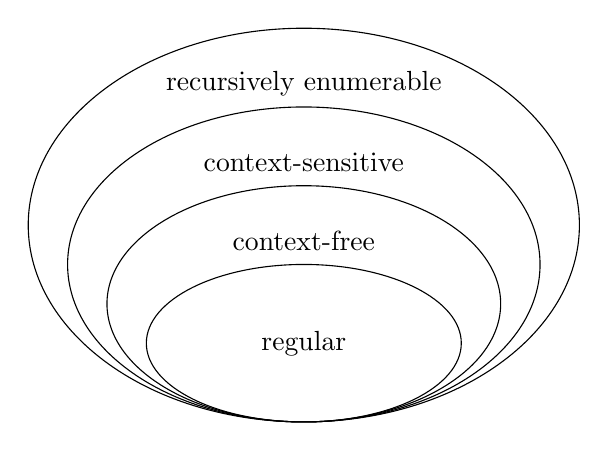
\begin{tikzpicture}
        \draw (0,0) ellipse (2 and 1);
        \draw (0,0.5) ellipse (2.5 and 1.5);
        \draw (0,1) ellipse (3 and 2);
        \draw (0,1.5) ellipse (3.5 and 2.5);

        \node at (0,0) {regular};
        \node at (0,1.3) {context-free};
        \node at (0,2.3) {context-sensitive};
        \node at (0,3.3) {recursively enumerable};
    \end{tikzpicture}
    \caption{Chomsky hierarchy of formal languages}
    \label{fig:chomsky-hierarchy}
\end{figure}


\subsubsection{Practical Implications}
\begin{itemize}
    \item \textbf{Regular Expressions}: Used in text processing (e.g., \texttt{grep}, lexical analyzers) \cite{kernighan1984unix, hopcroft2006introduction}.  
    \item \textbf{Context-Free Grammars}: Define programming language syntax (e.g., Python’s grammar) \cite{chomsky1956three, hopcroft2006introduction}.  
    \item \textbf{Closure Properties}: Enable decidability proofs (e.g., emptiness testing for DFAs) \cite{hopcroft2006introduction}.  
    \item \textbf{Stochastic Models}: Applied in natural language processing and speech recognition for probabilistic pattern matching \cite{rabin1963probabilistic}.  
\end{itemize}

\begin{figure}[h]
    \centering
    \begin{tikzpicture}[->,>=stealth,shorten >=1pt,auto,node distance=2.8cm,
        semithick, state/.style={circle, draw, minimum size=1.5cm}]
    
    \node[state, initial] (q0) {$q_0$};
    \node[state, accepting] (q1) [right of=q0] {$q_1$};
    
    \path 
    (q0) edge [loop above] node {$0$} (q0)
         edge [bend left] node {$1$} (q1)
    (q1) edge [loop above] node {$1$} (q1)
         edge [bend left] node {$0$} (q0);
    \end{tikzpicture}
    \caption{Example DFA recognizing even number of 1s}
    \label{fig:dfa-example}
\end{figure}

\subsubsection{Automata Definition Fundamentals}  
All automata share core structural components \cite{hopcroft2006introduction, chomsky1956three}.  

\begin{definition}[Classical Finite Automaton]
    \label{def:finite-automaton}
    A \textit{finite automaton} is a computational model that processes input symbols to recognize languages. Formally, a finite automaton $M$ is a quintuple $(Q, \Sigma, \delta, q_0, F)$, where:
    \begin{itemize}
        \item {States ($Q$)}: A finite set of configurations representing computational progress \cite{hopcroft2006introduction}. 
        \item {Input Alphabet ($\Sigma$)}: Defined symbols the automaton processes \cite{hopcroft2006introduction}.
        \item {Transition Function ($\delta$)}: Governs state changes based on input \cite{chomsky1956three}:  
        \begin{itemize}
            \item \textit{Deterministic}: $\delta: Q \times \Sigma \to Q$ (e.g., DFA) \cite{hopcroft2006introduction}.  
            \item \textit{Nondeterministic}: $\delta: Q \times \Sigma \to 2^Q$ (e.g., NFA) \cite{rabin1963probabilistic}.  
        \end{itemize}
        \item {Initial State ($q_0 \in Q$)}: The starting configuration \cite{hopcroft2006introduction}. 
        \item {Accept States ($F \subseteq Q$)}: Terminal states indicating successful computation \cite{hopcroft2006introduction}.
    \end{itemize} 
\end{definition}

\noindent\textit{Example}: The DFA in Figure \ref{fig:dfa-example} has:  
\begin{itemize}
    \item $Q = \{q_0, q_1\}$  
    \item $\Sigma = \{0, 1\}$  
    \item $\delta(q_0, 1) = q_1$, $\delta(q_1, 0) = q_0$ \textit{(partial specification)}  
    \item $F = \{q_1\}$ (accepts even number of 1s)  
\end{itemize}
\noindent\textbf{Graphical notation}: 
\begin{itemize}
    \item States: Circles with $q_i$ labels  
        \item Initial state: Arrow pointing to the state ($q_0$)  
        \item Accept states: Double circles ($q_1$ in \ref{fig:dfa-example})  
        \item Transitions: Directed edges labeled with input symbols  
\end{itemize}



\begin{table}[htbp]
    \centering
      \begin{tabular}{@{}lllll@{}}
          \toprule
          \textbf{Automaton} & \textbf{State Memory} & \textbf{Transition Type} & \textbf{Acceptance Condition} \\ \midrule
          DFA & None & Deterministic & Final state membership \cite{hopcroft2006introduction} \\
          NFA & None & Nondeterministic & Existence of accepting path \cite{hopcroft2006introduction} \\
          PDA & Stack & Deterministic/Nondet. & Final state + empty stack \cite{chomsky1956three} \\
          Turing Machine & Tape & Deterministic & Halting in accept state \cite{turing1936computable} \\
          \bottomrule
      \end{tabular}%
    \caption{Automata representation variations}
    \label{tab:automata-variations}
\end{table}